\chapter{Concepts of Wireguard}
  This chapter provide the core concepts of Wireguard protocol, especially in its handshake
  and timer state machine. Section \ref{w1} gives a high-level overview of the traits of the
  protocols, and the cryptography primitives that they build upon. 
  Section \ref{w2}  details the fondational handshake protocol that Wireguard's
  key exchange protocol builds upon. Section \ref{w3} defined all messages types of Wireguard and
  section \ref{w4} descibes the several timers constraint of Wireguard.
\section{Protocol \& Cryptography} \label{w1}
\subsection{Overview}
 Wireguard works as an encrypted IP network tunnel, resides at the layer 3 of the OSI layer, and
 uses UDP as its transport protocol. The establishment of a secure session before any 
 transmission of data is via 1-RTT key-exchange handshake protocols. This handshake protocol
 is designed based on a Trevor Perin's noise handshake pattern \cite{noise}. After the handshake, the  
 transported IP payload are protected using ChaCha20-Poly1305 Authenticated Encryption with 
 Associated Data (AEAD) \cite{rfc8439}.

 In Wireguard, the endpoints of communication have no role of server and client, but works in a
 peer-to-peer style. At any point in time, a peer can have a role of an \textbf{initator}, start to send 
 a handshake initiation message to create a secure channel with a \textbf{responder}. If the secure channel
 is not active for some amount of time, the initiator peer can change to a responder in the event of
 a the previous responder tries to initiate a new handshake, leading to the establishment of a new session
 between 2 peers. Figure \ref{fig:pwu_hs} illustrates this handshake flow with periodic key rotation.

\begin{figure}[h]
  \centering
  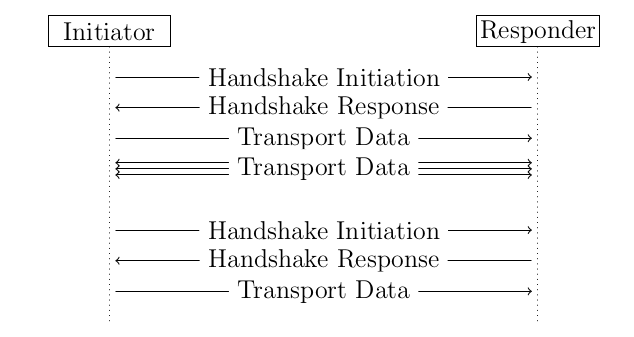
\includegraphics[width=0.8\linewidth]{pwu}
  \caption{After the handshake, both peers can send data towards each other. After a duration, rekeying occurs to create a new session. See \cite[p.~7]{pwu}}
  \label{fig:pwu_hs}
\end{figure}

 A static 32-byte Curve25519 \cite{curve} public key are used to identified an endpoint inside the tunnel. Without the
 proof of sender's knowledge on this public key, an endpoint will never respond. Thus, adversaries can't
 probe any system protected by Wireguard, using port scanning if they do not know the long-term static 
 public key.

The Wireguard handshake protocol can be considered as a 1.5 round-trip time (1.5-RTT) handshake \cite{pwu}. 
Upon the reception of the handshake response after sending a handshake initiation, the initiator
can promplty begin delivering encrypted payload. To safeguard against replay attacks, 
the responder must wait to send encrypted data messages until it has received an encrypted data 
message from the initiator, which serves as an acknowledgment of the handshake response.

During a handshake, new ephemeral key pairs will be generated by both parties, with the private key
being wiped after the handshake, assuring the forward secrecy of the session. Each session is bound
by fixed lifetime and the number of data messages that can be sent. When either of the limits is reached,
the derivation of new session keys are required if the peers want to extend the communication. The impact
of compromised session key is also mitigated by frequent periodic key rotation.

There is no direct shutdown signal within the protocol, only session removal after a fixed duration.
Even if one side has terminated its VPN tunnel, the peer would remain unaware and 
keep forwarding data.

Wireguard also provides an optional pre-shared symmetric key (PSK) mode, where any pairs of peer
pre-share a 256-bit symmetric encryption key between themselves, to assure the post-quantum 
security as long as the PSK never leaks out. This protection is against the idea that if 
adversaries may be recording all the traffic for a long time, until the quantum computer exists.
With PSK, despite the fact they maybe break all Curve25519-encrypted traffic, but not the ones that
include a PSK.

Another adversary model that Wireguard mititage is the denial of service through CPU exhaustion denial
of services attack \cite[p.~268]{cpu}. This mechanism is achieved via an encrypted cookie, when a peer is currently 
under load. This will be explained more in section \ref{iot:cookie}.

At last, Wireguard is cryptographically opinionated. The protocol intentionally does not provide 
any form of flexibility when it comes to choosing the cryptography suite, hence a negation for
cryptography algorithms does not exist. Specifically, Wireguard uses the following modern
cryptography constructions:
\begin{description}
  \item[Noise protocol framework]  A set of cryptographic handshake patterns that 
  serve as building blocks for creating new secure protocols with authenticated key agreement.
  \item[Elliptic Curve Diffie-Hellman (ECDH)] A Curve25519-based key-argeement protocol 
  with small key size and simple requirements regarding key validation.
  \item[ChaCha20-Poly1305] a modern AEAD combining ChaCha20 \cite{chacha20} stream cipher 
  and Poly1305 \cite{poly1305} authenticator to achieve authenticity and confidentiality. 
  \item[XChaCha-Poly1305] an extended version of chacha20-poly1305 that supports 192-bit nonce.
  This is used for cookie encryption \cite{irtf-cfrg-xchacha-03}.
  \item[HKDF] The HMAC-based Key Derivation Function \cite{rfc5869} to derive the encryption
  and decryption keys from the handshake state, keys and protocol messages.
  \item[BLAKE2] A fast and cryptographic hash function for message authentication code and is used
  by the HKDF \cite{rfc7693}.

\end{description}

\subsection{Cryptokey Routing}
  The binding between peers and the allowed source IP addresses is the fundamental principle to build 
  a secure VPN. As mentioned above, in Wireguard, peer must be identified by the 32-byte
  Curve25519 public key, allowing an association between the public key and the set
  of allowed IP addreses on the peer. This simple mapping is the concept behind the cryptokey
  routing table of Wireguard. A transmission of outbound packet will consult this table to search
  for the approriate public key, using the IP destination address of the packet. With inbound packets,
  after decryption and authentication, the source IP address need to be resolved to the same 
  peer that have the same public key used in the secure session for decrypting the packet. 
  In cryptokey routing table, each peer may optionally pre-specify an outer external IP address
  and UDP port of that peer's endpoint. If the endpoint is not specified, the external
  source IP of the machine will be used to determine the endpoint .
  This design also allow the peers to roam freely between different external IP addresses as the
  public is the main identification of the peer.
  
  Combining the roaming and the cryptokey routing table, when the network interface needs
  to send the data out, the flow start with the inspection of the IP destination of the packet 
  to find the corresponding peer and its public key (An ICMP "no route to host" will be returned
  in case of no peer). The packet is then encrypted with mentioned AEAD, prepended with
  extra headers and sent as a UDP packet to the internet. On the receiving flow, when a UDP packet
  is received, Wireguard finds the matching peer, decrypts the packet and updates the peers' endpoint.
  If the packet is either not an IP packet or there is no entry for source IP address of the packet
  inside the cryptokey routing table, the packet is droped. Otherwise, the packet will be dispatched
  to the layer above.
\section{Noise} \label{w2}
  Noise \cite{noise} is a framework to design secure protocol based on Diffie-Hellman(DH) key exchange \cite{dh}.
  With Noise, designers can construct new protocols that offer features such as identity hiding,
  mutual authentication, and forward secrecy for deriving shared symmetric keys. Furthermore, this
  framework has gone through formal analysis and verification \cite{noise_ex}. Although not all 
  Noise protocols ensure these security guarantees, the IKpsk2 form used by WireGuard does. 
  The rest of this section gives a general introduction to Noise, without focusing specifically on WireGuard.

  A Noise protocol begins with the exchange of \textbf{handshake messages} between two parties to
  generate a shared secret key for the encryption of \textbf{transport messages}. The first one
  to send the handshake message is refered to as the \textbf{initiator}, while the recipient of
  this message is called the \textbf{responder}.

  Each handshake in the Noise framework involves a long-term \textbf{static key pair} and/or
  \textbf{ephemeral key pair}. Every new handshake requires a fresh creation of the ephemeral
  keys. The static keys may be used for the purpose of authentication, when a peer has little
  information on the other's identity. Within the handshake, 256-bit \textbf{pre-shared symmetric key}
  can also be mixed in to bind the Noise session to a previous protocol-specific communication.
  Both the ephemeral and static keys are used in a chain of Diffie-Hellman computation to guarantee
  the forward secrecy. A cryptographic binding between the final shared secret and the handshake
  are achieved by the fact that all handshake messages and key material are used to derive
  the symmetric keys for handshake and the encryption of transport data.

  In Noise, the sequential exchange that comprises a handshake message is called a \textbf{handshake pattern}.
  Each handshake pattern consists of \textbf{message pattern}, which is arranged from a set of 
  pre-defined \textbf{tokens}. The tokens describes the modification to the cipher and handshake state, and
  data to read or write. The handshake state holds both local key pairs as well as the remote ephemeral 
  and static public keys of peer. The cipher state is made of a key and a counter-based nonce for 
  encryption, a handshake hash and a chaining key to derive the final symmetric key.  Noise framework 
  defines the following tokens for the message patterns:
  \begin{itemize}
    \item \textbf{e}: The sender creates a new ephemeral key pair, writes the public key into the 
    message buffer, and hashes this key into the handshake hash. In a PSK handshake, the chaining
    key is mixed with the ephemeral public key.
    \item \textbf{s}: The sender encrypts the static public key and write the result to message buffer. 
    if the handshake symmetric key exists, otherwise the plaintext of the public key will be written.
    The result will also be hashed into the handshake hash.
    \item \textbf{ee}, \textbf{es}, \textbf{se}, \textbf{ss}: DH computation is performed using
    the sender's ephemeral or static private key (determined by the first letter) and the receiver's
    ephemeral or static public key (determined by the second letter). The output is hashed into
    the chaining key, reseting the cipher state with a new key derived from the chaining key and 
    a zero nonce.
    \item \textbf{psk}: A pre-shared symmetric key is hashed both into the chaining key and the
    handshake hash state. As the chaining key derives the symmetric key directly, it's essential
    to mix the nonce into the chaining key for the generation of a randomized symmetric encryption
    key. This mitigates the key resuse vulnerability. The ephemeral public key provided by the "e" 
    token serves as this nonce. Consequently, in valid Noise protocols that utilize the \textbf{psk} token, 
    encryption must be preceded by the \textbf{e} token. An example of invalid pattern is 
    ``\textbf{psk}, \textbf{s}, \textbf{e}''. Here, \textbf{s} establishes the encrypted static
    public key with a fixed symmetric key derived from the PSK.
  \end{itemize}


The order of tokens within a message pattern is crucial. For instance, ``\textbf{s}, \textbf{ss}''
differs from ``\textbf{ss}, \textbf{s}''. In the former, the sender’s long-term static public key is presented 
in plain text (``\textbf{s}''), followed by a DH computation between the static keys of both parties (``\textbf{ss}''). 
Any subsequent messages following this pattern will be encrypted with derived keys. In contrast, 
the latter pattern (``\textbf{ss}, \textbf{s}'') indicates that the sender’s long-term static public key is encrypted, 
using keys derived from a hash that incorporates the DH computation between the two parties' static 
keys (``\textbf{ss}'').

Before the handshake, protocols may already possess information about the peer's static and/or 
ephemeral public keys. This knowledge is represented by one of the \textbf{pre-message patterns}: "\textbf{e}," "\textbf{s}," 
"\textbf{e}, \textbf{s}," or none if there are no pre-messages. The "\textbf{s}" pre-message 
pattern signifies knowledge of the other party's static public key, while the "\textbf{e}" pre-message pattern, 
used in a fallback scenario, indicates a previously shared fresh ephemeral public key. None of 
these public keys will be published again during the handshake; they remain implicit. 
The pre-message patterns and message patterns together create a \textbf{handshake pattern} that includes: 
\begin{itemize}
  \item A pre-message pattern for the initiator, which conveys information about the responder’s public keys.
  \item A pre-message pattern for the responder, which conveys information about the initiator’s public keys.
  \item A chain of message patterns the form the handshake messages. Each message pattern has a specific direction that influences how the tokens are interpreted. 
  For instance, for the initiator, the $\rightarrow$ \textbf{s} notation signifies sending the 
  initiator’s static public key, whereas the responder interprets it as reading the initiator’s 
  static public key.
\end{itemize}

Without knowledge of the exact public keys from the pre-message patterns, it will be 
impossible to derive the correct symmetric keys during the handshake. Consequently, 
this will lead to a failure of the handshake due to mismatched handshake states.


Noise specifies several standard handshake patterns, each with different requirements, 
properties, and security guarantees. Transmission of user data can happen after a completed
handshake or inside the buffer of message pattern within a handshake. Nevertheless, sending such
data beforehand can lead to reduced authenticity and confidentiality.

A instantiation of a concrete Noise protocol requires a choosing of \textbf{handshake pattern}, a
\textbf{DH function}, a \textbf{cipher function}, and a \textbf{hash function}. A prologue byte pattern 
can be established to associate the cryptographic keys with this value. Following is the instantiation
of Wireguard:
\begin{itemize}
  \item \textbf{handshake pattern}  IKpsk2
  \item \textbf{DH function} X25519
  \item \textbf{cipher function} ChaCha20-Poly1305
  \item \textbf{hash function} BLAKE2s
  \item \textbf{prologue} WireGuard v1 zx2c4 Jason@zx2c4.com
\end{itemize}

The name of the \textbf{IKpsk2} handshake pattern is explained as:
\begin{itemize}
  \item \textbf{I}: static public key is \textbf{i}mmediately transmitted to the
  responder, despite absent or reduced identity hiding.
  \item \textbf{K}: static public key for the responder is \textbf{k}nown to the initiator.
  \item \textbf{psk2}: a \textbf{PSK} is used at the end of the \textbf{second} handshake message.
\end{itemize}

The name for the Noise protocol is concatenated from the string Noise, the
handshake pattern, and functions, separated by an underscore ({\_}). Hence, for Wireguard,
the full Noise protocol name is:  Noise{\_}IKpsk2{\_}25519{\_}ChaChaPoly{\_}BLAKE2s.
The details of the IKpsk2 is presented in section \ref{ikpsk2}.

\subsection{IKpsk2 Handshake Pattern} \label{ikpsk2}
  The steps to execute the IKpsk2 handshake pattern used in Wireguard will be elaborated in this
  section. Following is the explaination for several operators, functions and symbols:
    \begin{itemize}
      \item $S^{pub}_i$: the initiator's 32-byte static public key.
      \item $E^{priv}_r$: the responder's 32-byte ephemeral private key.
      \item $Q$: optional 32-byte pre-shared symmetric key.
      \item $T^{send}_i$, $T^{recv}_r$: the initator's 32-byte transport data symmetric key for sending,
      and the responder's 32-byte transport data symmetric key for receiving.
    \end{itemize}

  The symbols for handshake and cipher state:
    \begin{itemize}
      \item $h$: the 32-byte handshake hash.
      \item $ck$: the 32-byte chaining key.
      \item $k$: the 32-byte handshake cipher key.
    \end{itemize}
  
  The functions and constants that will be used:
    \begin{itemize}
      \item \textbf{ECDH(private key, public key)}: the Elliptic Curve Diffie-Hellman function \cite{curve},
      returning the 32-byte shared secret from 32-byte public key and 32-byte private key.
      \item \textbf{ECDH$\_$GEN()}: returns a key pairs consisting of a random Curve25519 private key and
      the related public key.
      \item \textbf{AEAD$\_$ENC(cleartext, aad, key, nonce)}: applies ChaCha20-Poly1305 AEAD encryption
      on a variable-length cleartext message, using a 256-bit key, a 96-bit counter after prepending the 64-bit nonce
      with 4 bytes of zero and arbitary length additional authenticated data to return the ciphertext
      including a 16-byte authentication tag.
      \item \textbf{AEAD$\_$DEC(ciphertext, aad, key, nonce)}: the reverse of \textbf{AEAD$\_$ENC} that
      authenticates and decrypt the ciphertext to return the original plaintext.
      \item \textbf{Hash(data)}: hashes the variable-length data with BLAKE2s function to return
      32 bytes of output.
      \item \textbf{KDF$_n$(key, input)}: derives the n 32-bytes keys with HKDF, using unkeyed 
      BLAKE2s as the hash function for the HMAC \cite[section 13.2]{crypto}. The construction of
      HKDF is as follow:
      \begin{align*}
        PRK  &= HMAC(key, input) \\
        T_1  &= HMAC(PRK, 0x1) \\
        T_2  &= HMAC(PRK, T_1 || 0x2) \\
        &\dots \\
        T_n  &= HMAC(PRK, T_{n - 1} || n)
    \end{align*}
    \end{itemize}

    The IKpsk2 handshake pattern in compact notation are shown Figure \ref{fig:ikpsk}. The details of the
    computation follows below, as a reiteration in \cite[p.~15]{pwu}.

  \begin{figure}[h]
    \begin{center}
      \begin{varwidth}{\textwidth}
      \large IKpsk2:
      \begin{enumerate}
          \item \(\leftarrow s\) \\
          \(\dots\)
          \item \(\rightarrow e, es, s, ss\)
          \item \(\leftarrow e, ee, se, psk\)
      \end{enumerate}
      \end{varwidth}
    \end{center}
    \caption{Compact notation for IKpsk2. The dots distinguish between pre-messages and messages. See \cite[p.~36]{noise}}
    \label{fig:ikpsk}
  \end{figure}

  \newcounter{cnt}
  \setcounter{cnt}{1}
  The hashing of protocol name and prologue begins the handshake computation.
    \begin{center}
      \begin{varwidth}{\textwidth}
      \begin{enumerate} [start = \value{cnt}]
          \item $h_0$ = \textbf{Hash}(``Noise IKpsk2 25519 ChaChaPoly BLAKE2s'')
          \item $ck_0$ = $h_0$
          \item $h_1$ = \textbf{Hash}($h_0$ $\Vert$ ``WireGuard v1 zx2c4 Jason@zx2c4.com'')
          \addtocounter{cnt}{3}
      \end{enumerate}
      \end{varwidth}
    \end{center}
  
  Next, the handshake messages and pre-messages will be processed. Since there are message tokens
  that have different interpretation depending on the initator and the responder, I: and R: will
  be prefixed before the line to constratin them to the initator or responder correspondingly.
  Following are how to interpret the three (pre-)messages from Figure \ref{fig:ikpsk}:

  \newcounter{msg}
  \setcounter{msg}{0}
  \begin{enumerate} [start = \value{msg}]
    \item $\leftarrow$ s: a pre-message from responder to initiator, with ``s'' as the
    previously out-of-band exchanged static public key $S^{pub}_r$.
    \addtocounter{msg}{1}
  \end{enumerate}

    \begin{center}
      \begin{varwidth}{\textwidth}
      \begin{enumerate} [start = \value{cnt}]
          \item $h_2$ = \textbf{Hash}($h_1$ $\Vert$ $S^{pub}_r$)
          \addtocounter{cnt}{1}
      \end{enumerate}
      \end{varwidth}
    \end{center}

  \begin{enumerate} [start = \value{msg}]
    \item $\rightarrow$ e, es, s, ss: the initiator's message to the responder:
    \addtocounter{msg}{1}
    \begin{itemize}
      \item ``e'': the initator creates an ephemeral key pair, transmits the public key
      $E^{pub}_i$ to the responder. $E^{pub}_i$ is mixed into the handshake hash and the chaining
      key because of the PSK.
      \begin{center}
        \begin{varwidth}{\textwidth}
          \begin{description}
          \item[\textnormal{\arabic{cnt}}.] I: ($E^{priv}_i$, $E^{pub}_r$) = \textbf{ECDH{\_}GEN()}; write $E^{pub}_i$ \\
                R:  read $E^{pub}_i$
          \addtocounter{cnt}{1}
          \item[\textnormal{\arabic{cnt}}.] $h_3$ = \textbf{Hash}($h_2$ $\Vert$ $E^{pub}_i$)
          \addtocounter{cnt}{1}
          \item[\textnormal{\arabic{cnt}}.] $ck_1$ = \textbf{KDF}$_1$($ck_0$, $E^{pub}_i$)
          \addtocounter{cnt}{1}
          \end{description}
        \end{varwidth}
      \end{center}
    \item ``es'':  the responder calculates the $es = \textbf{ECDH}(S^{priv}_r, E^{pub}_i)$. The
    same shared secret is calculated as $es = \textbf{ECDH}(E^{priv}_i, S^{pub}_r)$ for the initiator.
      \begin{center}
        \begin{varwidth}{\textwidth}
          \begin{description}
          \item[\textnormal{\arabic{cnt}}.] 
                I: ($ck_2$, $k_0$) = \textbf{KDF}$_2$($ck_1$, \textbf{ECDH}($E^{priv}_i$, $S^{pub}_r$)) \\
                R: ($ck_2$, $k_0$) = \textbf{KDF}$_2$($ck_1$, \textbf{ECDH}($S^{priv}_r$, $E^{pub}_i$))
                % R:  read $E^{pub}_i$
          \addtocounter{cnt}{1}
          \end{description}
        \end{varwidth}
      \end{center}

    \item ``s'':  the initiator transmits its encrypted static public key $S^{pub}_i$. On failure of
    decryption, the handshake is aborted.
      \begin{center}
        \begin{varwidth}{\textwidth}
          \begin{description}
          \item[\textnormal{\arabic{cnt}}.] 
                I: msg = \textbf{AEAD{\_}ENC}($S^{pub}_i$, $h_3$, $k_0$, 0); write msg \\
                R: $S^{pub}_i$ = \textbf{AEAD{\_}DEC}(msg, $h_3$, $k_0$, 0); abort on failure
          \addtocounter{cnt}{1}
          \item[\textnormal{\arabic{cnt}}.] $h_4$ = \textbf{Hash}($h_3$ $\Vert$ $msg$)
          \addtocounter{cnt}{1}
          \end{description}
        \end{varwidth}
      \end{center}

    \item ``ss'':  the responder calculates the $ss = \textbf{ECDH}(S^{priv}_r, S^{pub}_i)$. The
    same shared secret is calculated as $ss = \textbf{ECDH}(S^{priv}_i, S^{pub}_r)$ for the initiator.
      \begin{center}
        \begin{varwidth}{\textwidth}
          \begin{description}
          \item[\textnormal{\arabic{cnt}}.] 
                I: ($ck_3$, $k_1$) = \textbf{KDF}$_2$($ck_2$, \textbf{ECDH}($S^{priv}_i$, $S^{pub}_r$)) \\
                R: ($ck_3$, $k_1$) = \textbf{KDF}$_2$($ck_2$, \textbf{ECDH}($S^{priv}_r$, $S^{pub}_i$))
          \addtocounter{cnt}{1}
          \end{description}
        \end{varwidth}
      \end{center}
    \item Add an encrypted (possibly) empty payload to the message buffer in the handshake. If the
    decryption fails for the responder, it stops the handshake. For Wireguard, the payload is
    the current timestamp.
    \begin{center}
      \begin{varwidth}{\textwidth}
        \begin{description}
        \item[\textnormal{\arabic{cnt}}.] 
              I: c = \textbf{AEAD{\_}ENC}(time, $h_4$, $k_1$, 0); write c \\
              R: time = \textbf{AEAD{\_}DEC}(c, $h_4$, $k_1$, 0); abort on failure
        \addtocounter{cnt}{1}
        \item[\textnormal{\arabic{cnt}}.] $h_5$ = \textbf{Hash}($h_4$ $\Vert$ $m$)
        \addtocounter{cnt}{1}
        \end{description}
      \end{varwidth}
    \end{center}
  \end{itemize}
  \end{enumerate}


  \begin{enumerate} [start = \value{msg}]
    \item $\leftarrow$ e, ee, se, psk: the responder's message to the initiator:
    \addtocounter{msg}{1}
    \begin{itemize}
      \item ``e'': the responder creates an ephemeral key pair, transmits the public key
      $E^{pub}_r$ to the initator. $E^{pub}_r$ is mixed into the handshake hash and the chaining
      key because of the PSK.
      \begin{center}
        \begin{varwidth}{\textwidth}
          \begin{description}
          \item[\textnormal{\arabic{cnt}}.] R: ($E^{priv}_r$, $E^{pub}_i$) = \textbf{ECDH{\_}GEN()}; write $E^{pub}_r$ \\
                I:  read $E^{pub}_r$
          \addtocounter{cnt}{1}
          \item[\textnormal{\arabic{cnt}}.] $h_6$ = \textbf{Hash}($h_5$ $\Vert$ $E^{pub}_r$)
          \addtocounter{cnt}{1}
          \item[\textnormal{\arabic{cnt}}.] $ck_4$ = \textbf{KDF}$_1$($ck_3$, $E^{pub}_r$)
          \addtocounter{cnt}{1}
          \end{description}
        \end{varwidth}
      \end{center}
    \item ``ee'':  the responder calculates the $ee = \textbf{ECDH}(E^{priv}_r, E^{pub}_i)$. The
    same secret is calculated as $es = \textbf{ECDH}(E^{priv}_i, E^{pub}_r)$ for the initiator.
      \begin{center}
        \begin{varwidth}{\textwidth}
          \begin{description}
          \item[\textnormal{\arabic{cnt}}.] 
                R: $ck_5$ = \textbf{KDF}$_1$($ck_4$, \textbf{ECDH}($E^{priv}_r$, $E^{pub}_i$)) \\
                I: $ck_5$ = \textbf{KDF}$_1$($ck_4$, \textbf{ECDH}($E^{priv}_i$, $E^{pub}_r$))
          \addtocounter{cnt}{1}
          \end{description}
        \end{varwidth}
      \end{center}

  \item ``se'':  the responder calculates the $se = \textbf{ECDH}(E^{priv}_r, S^{pub}_i)$. The
  same secret is calculated as $se = \textbf{ECDH}(S^{priv}_i, E^{pub}_r)$ for the initiator.
    \begin{center}
      \begin{varwidth}{\textwidth}
        \begin{description}
        \item[\textnormal{\arabic{cnt}}.] 
              R: $ck_6$ = \textbf{KDF}$_1$($ck_5$, \textbf{ECDH}($E^{priv}_r$, $S^{pub}_i$)) \\
              I: $ck_6$ = \textbf{KDF}$_1$($ck_5$, \textbf{ECDH}($S^{priv}_i$, $E^{pub}_r$))
        \addtocounter{cnt}{1}
        \end{description}
      \end{varwidth}
    \end{center}

    \item ``psk'':  include the pre-shared symmetric key $Q$ in both chaining key and the
    handshake hash.
    \begin{center}
        \begin{varwidth}{\textwidth}
          \begin{description}
          \item[\textnormal{\arabic{cnt}}.] ($ck_7$, $\tau$, $k_2$) = \textbf{KDF}$_3$($ck_6$, $Q$)
          \addtocounter{cnt}{1}
          \item[\textnormal{\arabic{cnt}}.] $h_7$ = \textbf{Hash}($h_6$ $\Vert$ $\tau$)
          \addtocounter{cnt}{1}
          \end{description}
        \end{varwidth}
      \end{center}

    \item Add an encrypted (possibly) empty payload to the message buffer in the handshake. If the
    decryption fails for the responder, it aborts the handshake.
    \begin{center}
      \begin{varwidth}{\textwidth}
        \begin{description}
        \item[\textnormal{\arabic{cnt}}.] 
              R: c = \textbf{AEAD{\_}ENC}(m, $h_7$, $k_2$, 0); write c \\
              I: m = \textbf{AEAD{\_}DEC}(c, $h_7$, $k_2$, 0); abort on failure
        \addtocounter{cnt}{1}
        \item[\textnormal{\arabic{cnt}}.] $h_8$ = \textbf{Hash}($h_7$ $\Vert$ $m$)
        \addtocounter{cnt}{1}
        \end{description}
      \end{varwidth}
    \end{center}
  \end{itemize}
  \end{enumerate}

  At last, the handshake ends with the derivation of the symmetric keys for transport data encryption,
  using HKDF with the chaining key and a empty string $\epsilon$.
    \begin{center}
      \begin{varwidth}{\textwidth}
        \begin{description}
        \item[\textnormal{\arabic{cnt}}.] 
              I: ($T^{send}_i$, $T^{recv}_i$) = \textbf{KDF}$_2$($ck_2$, $\epsilon$) \\
              R: ($T^{send}_r$, $T^{recv}_r$) = \textbf{KDF}$_2$($ck_2$, $\epsilon$)
        \addtocounter{cnt}{1}
        \end{description}
      \end{varwidth}
    \end{center}

  This wraps up the execution and overview of the Noise IKpsk2 protocol. Next section will delve 
  into how Wireguard uses this pattern for its payload.

\section{Wireguard Messages} \label{w3}
    This sections details the underlying Wireguard messages that realizes the Noise handshake protocol,
    protects again denial of service attacks and encapsulates the IP packet in a robust tunnel. In  
    Wireguard, there are four kinds of message, all of which start with a single type byte, followed
    by three zero reserved bytes. This layout allows the implementation to read the first 4 bytes
    of the message as a little-endian integer. 
    
    \begin{figure}[h]
      \centering
      \begin{subfigure}[b]{0.6\textwidth}
          \centering
          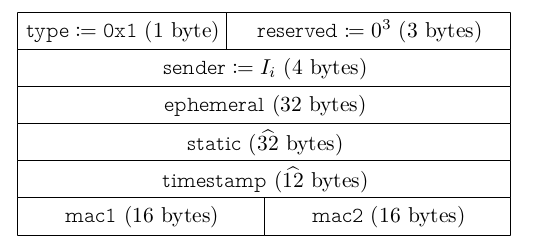
\includegraphics[width=\textwidth]{hs_init}
          \caption{Handshake Initiation}
          \label{fig:hsinit}
      \end{subfigure}
      \hfill
      \begin{subfigure}[b]{0.6\textwidth}
          \centering
          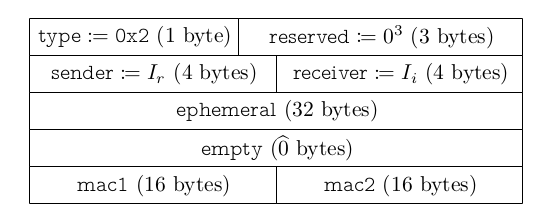
\includegraphics[width=\textwidth]{hs_resp}
          \caption{Handshake Response}
          \label{fig:hsresp}
      \end{subfigure}
      \caption{Handshake messages, see \cite[p.~10]{wireguard}.}
      \label{fig:hs}
    \end{figure} 

    Figure \ref{fig:hs} show first 2 types of Wireguard messages: \textbf{Handshake initiation} and
    \textbf{Handshake response}. These 2 messages are the adaptation of Wireguard for Noise
    handshake. Both of messages contains a \textbf{sender index} to indicate a 32-bit index
    that locally represents the sending peer. The \textbf{receiver index} of handshake response
    is the received \textbf{sender index} from the initiator. The ephemeral fields are the
    ephemeral public keys for key exchange, while the static field of the \textbf{handshake initiation}
    is the encrypted static public key of the initator after the DH computation. The initiation message
    also includes an encrypted TAI64N \cite{tai64} timestamp to protect against replay attack. The motivation
    for the final MAC fields are explained in section \ref{iot:cookie}. These MAC fields are computed
    using the keyed BLAKE2s MAC with a 16-byte hash value as output. Depending on the recipient and
    field type, the input and key for each MAC field will be different. To be specific:
      \begin{description}
        \item[MAC1] Using $S^{pub}_{m'}$ as the receiver static public key, the key of the MAC computation
        is the value: \textbf{Hash}(``mac1\texttt{----}'' $\Vert$ $S^{pub}_{m'}$). The input of the MAC is all
        the bytes of the message prior to MAC1 field.
        \item[MAC2] Given that the latest cookie was received within 120 seconds, this cookie
        would be the MAC2 key. Otherwise, if the key is too old or there is no such cookie, the MAC2 
        field will be zeroed out. The data for MAC2 is all the bytes prior to the MAC2 field.
      \end{description}
    
   The third type of message is the \textbf{Cookie Reply Message}, which is sent when the current
   peer is under load. The exact condition to transmit this cookie message is after the reception
   of a handshake message with valid MAC1 but invalid/expired  MAC2 and the peer is under load.
   The format of the message is as follow:

    \begin{figure}[h]
      \centering
      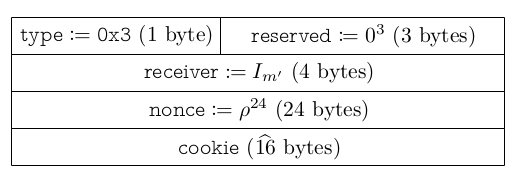
\includegraphics[width=0.7\textwidth]{cookie}
      \caption{Cookie Reply Message, see \cite[p.~13]{wireguard}.}
      \label{fig:cookie}
    \end{figure} 

    The receiver is the sender from the previous handshake message. With a random secret value $R_m$ that changes
    every two minutes, the concatenation of the last message's external IP source address and its 
    UDP source port, and MAC1 as M, the encrypted cookie is created like below:

    \begin{align*}
      \tau &= \textbf{BLAKE2s}(R_m, A_{m'}) \\
      cookie &= \textbf{XAEAD}(\tau, M, \textbf{Hash}(''cookie\texttt{--}'' \Vert S^{pub}_m), nonce)
    \end{align*}

    By using M as the additional authenticated data field, the cookie reply is securely bound 
    to the corresponding message, preventing peers from being targeted by fraudulent cookie 
    reply attacks. Additionally, this message is smaller than both the handshake initiation and 
    handshake response messages, reducing the risk of amplification attacks.

    The final type of messages is the Transport Data Message - the encrypted encapsulated payload
    for secure communication. A counter is included in the packet to use as the nonce for AEAD
    and a tool to prevent replay attack. The inner IP packet will padded with zero bytes until
    its length is a multiple of 16 to achieve a better address alignment, thus improving the
    performance on many CPU architectures.

    \begin{figure}[h]
      \centering
      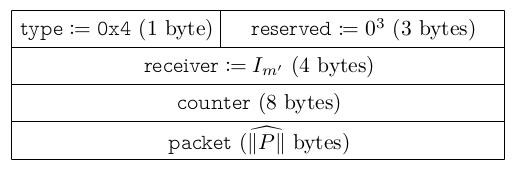
\includegraphics[width=0.6\textwidth]{dat}
      \caption{Transport Data Message, see \cite[p.~12]{wireguard}.}
      \label{fig:transdata}
    \end{figure} 


\section{Timers} \label{w4}
The Wireguard protocol leverages a simple timer state machine behind the scenes for the 
maintenance of session states, perfect forward secrecy and handshakes. The involved constants
for the timer state are as below:

\begin{center}
  \begin{tabular}{|c | c|} 
   \hline
   Symbol & Value \\
   \hline\hline
   \uppercase{Rekey-Afer-Messages} & $2^{60}$ messages \\ 
   \hline
   \uppercase{Reject-After-Messages} & $2^{64} - 2^{13} - 1$ messages \\
   \hline
   \uppercase{REKEY-AFTER-TIME} & 120 seconds \\
   \hline
   \uppercase{reject-after-time} & 180 seconds \\
   \hline
   \uppercase{rekey-attempt-time} & 90 seconds \\
   \hline
   \uppercase{rekey-timeout} & 5 seconds \\
   \hline
   \uppercase{keepalive-timeout} & 10 seconds \\
   \hline
  \end{tabular}
  \end{center}

  With multiple peers can be configured to be accepted on a host, the following are the constraints
  applied on a per-peer basis for the handshake initiation:
  \begin{enumerate}
    \item There can only be one handshake initiation sent every \uppercase{REKEY-TIMEOUT}.
    \item If there is no handshake response reception of a handshake initiation after \uppercase{rekey-timeout},
    a new handshake initiation will be constructed and transmitted again. This attempt happens
    for \uppercase{REKEY-attempt-time} seconds. This timer will be reset when a transport data
    message is ready to be sent.
    \item The handshake completion marks the starting of the age of a secure session. For the initator,
    this age begins when the processing of handshake reponse is done and the symmetric keys have
    been derived. For the responder, it is when the first valid transport data is received from
    the initiator.
    \item The only cause for a new handshake initiation is the transport data, no timer expiration
    should trigger it.
    \item A session that is older than \uppercase{reject-after-time} or has sent more than \uppercase{REJECT-AFTER-MESSAGES}
    is not usable.
    \item A handshake initiation may be sent after sending \uppercase{Rekey-after-messages}.
    \item After the initator sends data and the \uppercase{Rekey-after-time} has passed, 
    a new handshake initiation will be sent.
    \item After the initator receives data and the \uppercase{Reject-after-time} - \uppercase{keepalive-timeout} 
    - \uppercase{rekey-timeout} has passed, a new handshake initiation will be sent.


  \end{enumerate}